\documentclass[12pt, a4paper]{paper}
\usepackage{natbib}
\usepackage{graphicx}
\usepackage[noend]{algpseudocode}
\usepackage{algorithm}
\usepackage[demo]{graphicx}
\usepackage{babel,blindtext}

\title{\textbf{Clustering and Unsupervised Learning \\ Final Course Project}}
\author{Submitted by: Dor Litvak}
\date{Spring 2020}

\begin{document}

%%%%%%%%%%%%%%%%%%%%%%%%%%%%%%%%

\maketitle



\begin{figure}[h!]
\centering

\includegraphics[scale=0.1]{bgu.png} \\
\textbf{Ben-Gurion University of The Negev} 
\end{figure}

\newpage
%%%%%%%%%%%%%%%%%%%%%%%%%%%%%%%%


\section*{The Clustering problem}

The Clustering problem is the task of grouping a set of objects in such a way that objects in the same cluster are more similar to each other than to those in other clusters. \\
Formally, assuming N data points $x_{1}, ... x_{N}$ generated from K Gaussian's with $\theta_{1} = (\mu_{1}, \Sigma_{1}), ... , \theta_{K} = (\mu_{K}, \Sigma_{K})$. The prior probability $P(w_{i})$ and the classes conditional densities $P(x|w_{i}, \theta_{i})$\\
The assignment is to find the correct labels $y_{1}, ... y_{N}$, such that $\forall j \in (1,...,K)$ and  $\forall i$ when $x_{i} \sim N(\mu_{i}, \Sigma_{i})$ the label of $x_{i}$ would be: $y_{i} = j$ .\\ 

There are different types of clustering problems and thou different solutions.
The problems are differ from one another in the given information we have:
Does the number of clusters known? $\theta_{i}$ known? The $P(w_{i}), P(x|w_{i}, \theta_{i})$ known? \\ 

As you can see in Figure \ref{figure:Clustering Flowchart} Flowchart, if we know K - the number of classes the The prior probability $P(w_{i})$ and the classes conditional densities $P(x|w_{i}, \theta_{i})$ we can use simple Bayes Decision Theory Classification to find $y_{1}, ... y_{N}$ and $\theta_{1} ,...,\theta_{K}$ using the following formula: \\
$P(x|\theta) = \sum_{j=1}^{K}{P(x|w_{i}, \theta_{i})P(w_{i})}$ where $\theta = \theta_{1} ,...,\theta_{K}$ , $x = x_{1}, ... x_{N}$ \\
But, if we do not have the information above, we are getting to the left side of the flowchart, and assume we have an available data set. \\  
Now we are moving to the next question in the flowchart, and the main question in the field of the clustering problem do we have Pre-classification. 
\begin{itemize}
    \item Supervised Learning, the data set is classified. We will not discuss farther about Supervised Learning the second case is more interasting. 
    \item Unsupervised Learning, the data set is not classified. So we don't know the labels $y_{1}, ... y_{N}$. 
\end{itemize}
\textbf{Unsupervised Learning} the next two questions will help us to decide which Unsupervised Clustering method to use.
\begin{enumerate}
    \item Do we know the probability density function nature, meaning we know if the data came from Gaussian / Gamma / Cauchy / Beta / Poisson / etc distribution ? 
    \item Do we have a partition criteria?
\end{enumerate} 
\textit{If the answer to 1 is yes:} We can use on of the Expectation Maximization / Maximum Likelihood Estimation algorithms, we will further discuss on both. \\
\textit{If the answer to 1 is no and the answer to 2 is yes:} We can use Hard C-means / Fuzzy C-means / Deterministic Annealing , we will further discuss on them too. \\
\textit{If the answer to 1 is no and the answer to 2 is no:} We will use graphical clustering such Hierarchic Clustering / Minimum distance Clustering / Density Estimation / Self-Organizing Feature Maps. 

\begin{figure}[h!]
\centering
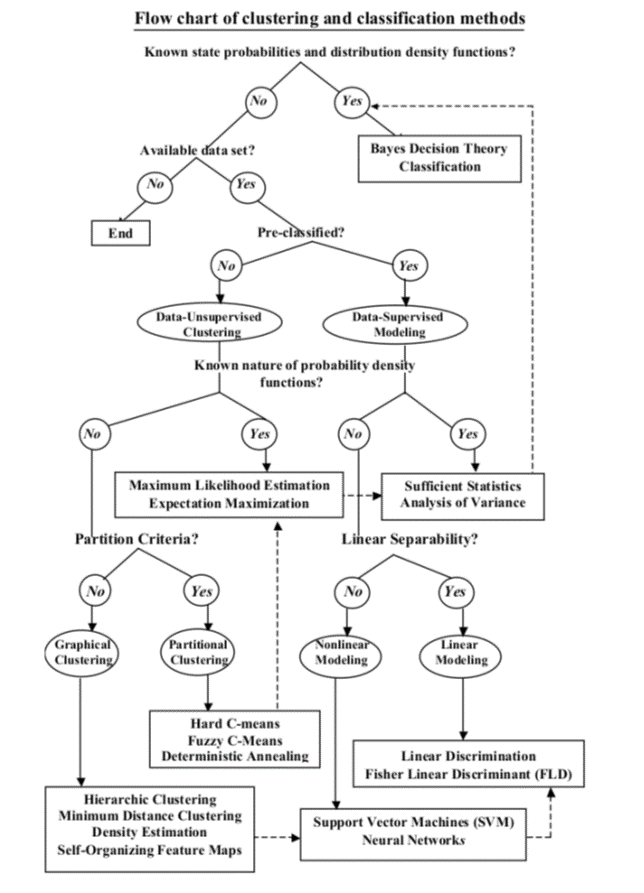
\includegraphics[scale=0.9]{clustering.png} \\
\caption{Clustering Flowchart}
\label{figure:Clustering Flowchart}
\end{figure}

\newpage
%%%%%%%%%%%%%%%%%%%%%%%%%%%%%%%%

\section*{Assignment 0 - Create the data}
In the first assignment we were asked to create a diverse data to tests the clustering assignment over.

\subsection*{2D random data}
Randomize data taken from c (constant number chosen) clusters with dots - number of data points in each cluster. the values of c, dots can easily change. 
The data point are draw from Gaussian distribution with random parameters mu and sigma different for each cluster.

\begin{figure}[h!]
\centering
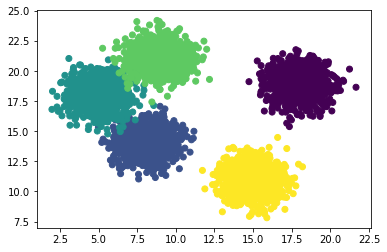
\includegraphics[scale=0.6]{5_c_1000_dots_20_scale.png}
\caption{5 clusters with 1000 random data points each and axis scale 20}
\label{fig:2D_1}
\end{figure}


\begin{figure}[h!]
\centering
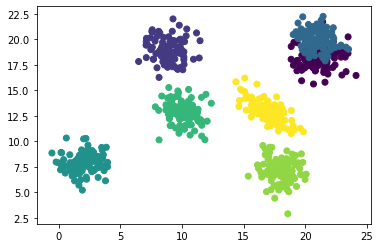
\includegraphics[scale=0.6]{7_c_100_dots_20_scale.png}
\caption{7 clusters with 100 random data points each and axis scale 20}
\label{fig:2D_2}
\end{figure}


\subsection*{3D random data}
Randomize data taken from c (constant number chosen) clusters with dots - number of data points in each cluster. the values of c, dots can easily change. 
The data point are draw from Gaussian distribution with random parameters mu and sigma different for each cluster.

\begin{figure}[h!]
\centering
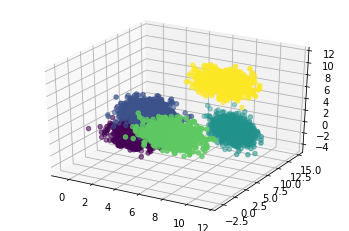
\includegraphics[scale=0.7]{c_5_1000_dots_spred_10.png}
\caption{5 clusters with 1000 random data points each and axis scale 10}
\label{fig:3D_1}
\end{figure}


\begin{figure}[h!]
\centering
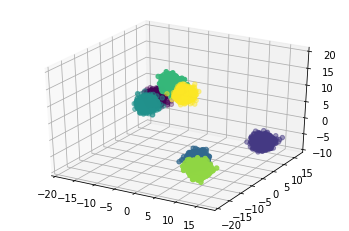
\includegraphics[scale=0.7]{c_7_dos_1000_spred_15.png}
\caption{7 clusters with 1000 random data points each and axis scale 15}
\label{fig:3D_2}
\end{figure}


\subsection*{IRIS data set}
The data set consists of 50 samples from each of three species of Iris (Iris setosa, Iris virginica and Iris versicolor). Four features were measured from each sample: the length and the width of the sepals and petals, in centimeters. Based on the combination of these four features, we want to distinguish the species from each other.

\begin{figure}[h!]
\centering
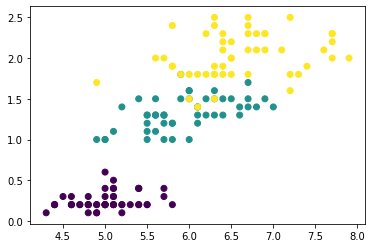
\includegraphics[scale=0.6]{iris_features_0_3.png}
\caption{Using the first and third features to distinguish between the iris sample}
\label{fig:iris_1}
\end{figure}

\begin{figure}[h!]
\centering
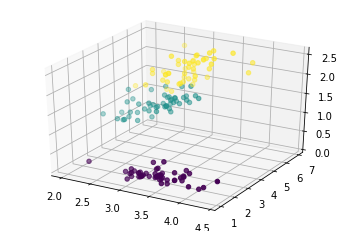
\includegraphics[scale=0.7]{iris_features_1_2_3.png}
\caption{Using the first, second and third features to distinguish between the iris sample}
\label{fig:iris_2}
\end{figure}

\newpage
%%%%%%%%%%%%%%%%%%%%%%%%%%%%%%%%

\begin{figure}[h!]
\centering
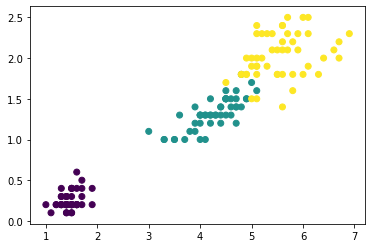
\includegraphics[scale=0.6]{iris_features_2_3.png}
\caption{Using the second and third features to distinguish between the iris sample}
\label{fig:iris_3}
\end{figure}

\begin{figure}[h!]
\centering
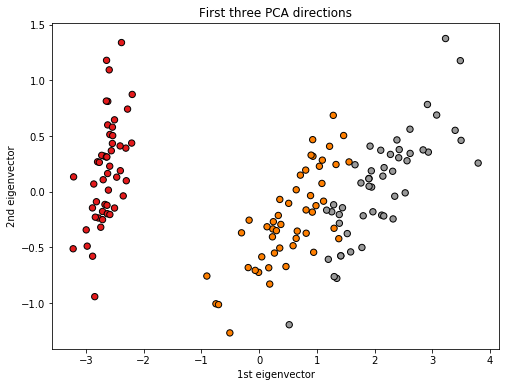
\includegraphics[scale=0.4]{iris_with_PCA_2_eigenvectors.png}
\caption{Using PCA to dimensionality reduction and taking the 2 eigenvectors correspond with the 2 largest eigenvalues}
\label{fig:iris_3}
\end{figure}


\subsection*{Circular Data}
Another interesting data is a circular data, with 2 or 3 rings (could be more, just for the example) in order to test how different methods will deal with this kind of data. 
In the figure circles with the same center (5,5), the first one with radius 1.5-1.7, the second with radius 1-1.2, the third with radius 0.2-0.5.
\begin{figure}[h!]
\centering
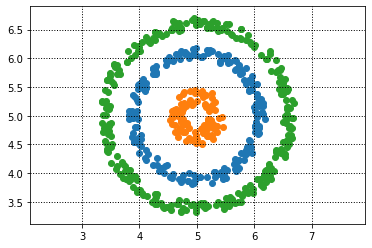
\includegraphics[scale=0.7]{circle.png}
\caption{Three random data taken from circles}
\label{fig:circles}
\end{figure}


\section*{Assignment 1 - Maximum likelihood estimation}

Maximum likelihood estimation is a method of estimating the parameters of a probability distribution by maximizing the likelihood function, so that under the assumed statistical model the observed data is most probable.

Formally (we will use 2D for the explanation but it could be 3D as well), Given n data points $(x_{1}, y_{1}),...,(x_{n},y_{n})$ we wish to classify those data points to c different clusters when c is fixed number as we choose. 

For the local Maximum likelihood estimate $\hat{\mu}_{i}, \hat{\Sigma}_{i}, \hat{P}(w_{i})$:

\begin{equation}
\hat{P}(w_{i}) = \frac{1}{n} \Sigma_{k=1}^n \hat{P}(w_{i}|x_{k}, \hat{\theta})
\end{equation}

\begin{equation}
\hat{\mu}_{i} = \frac
{\Sigma_{k=1}^n \hat{P}(w_{i}|x_{k}, \hat{\theta})x_{k}}
{\Sigma_{k=1}^n \hat{P}(w_{i}|x_{k}, \hat{\theta})} 
\end{equation}

\begin{equation}
\hat{\Sigma}_{i} = \frac
{\Sigma_{k=1}^n \hat{P}(w_{i}|x_{k}, \hat{\theta})(x_{k}-\mu_{i})(x_{k}-\mu_{i})^{t}}
{\Sigma_{k=1}^n \hat{P}(w_{i}|x_{k}, \hat{\theta})} 
\end{equation}


\begin{equation}
\hat{P}(w_{i}|x_{k}, \hat{\theta}) = \frac
{p(x_{k}|w_{i},\hat{\theta}_{i})\hat{P}(w_{i})}
{\Sigma_{j=1}^{c} p(x_{k}|w_{j},\hat{\theta}_{j})\hat{P}(w_{j})} 
\end{equation}

\newpage
%%%%%%%%%%%%%%%%%%%%%%%%%%%%%%%%


\begin{algorithm}
{\fontsize{10pt}{10pt}\selectfont
\caption{Maximum likelihood estimation}\label{alg:BrothForce}
\begin{algorithmic}[1]
\State Choose centers randomly*: $\mu_{i} \gets rand(x_{i}, y_{i})$.
\State Initialize covariance matrix  $\Sigma_{i} \gets rand\_spd\_matrix(2,2)$.
\State Initialize $\hat{P(w_{i})} \gets \frac{1}{c}$ 
\While {Run until convergence}
\State $\hat{P}(w_{i}|x_{k}, \hat{\theta}) \gets \forall i,k$ calculate the probability data point k came from center i: Eq.4 
\State Use $\hat{P}(w_{i}|x_{k}, \hat{\theta})$ to update $\hat{\mu}_{i}, \hat{\Sigma}_{i}, \hat{P}(w_{i})$ using Eq.1,2,3
\EndWhile 
\end{algorithmic}
}
\end{algorithm} 
*choose c data points to be centers, choose random values in the data range, etc... 

\subsection*{Results}
\textbf{Over 2D data points randomly drawn from 4 Gaussian's}
We initialize the MLE algorithm with randomly chosen from the data points centers .

\begin{figure}[h!]
\centering
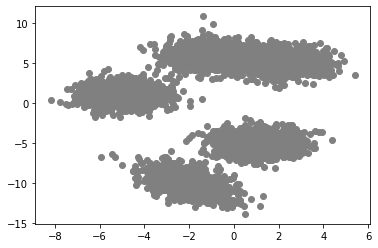
\includegraphics[scale=0.6]{MLE_2D_init.png}
\caption{Data taken from 5 different Gaussian's with 1000 data points taken from each one.}
\label{fig:MLE_1}
\end{figure}

\newpage
%%%%%%%%%%%%%%%%%%%%%%%%%%%%%%%%

\begin{figure}[h!]
\centering
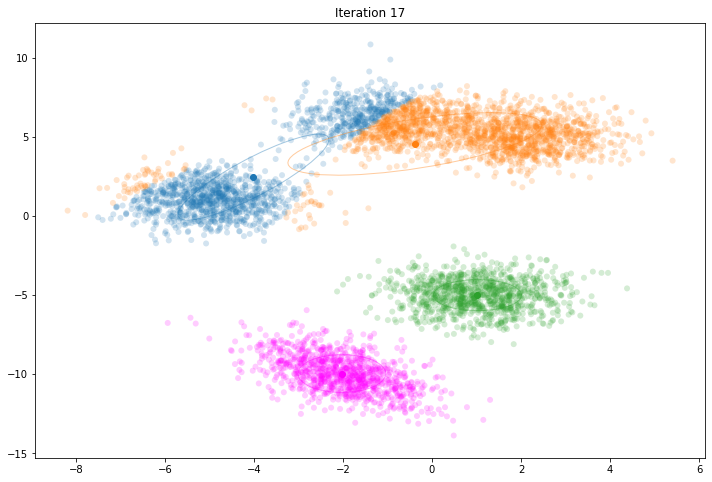
\includegraphics[scale=0.4]{MLE_iter_17.png}
\caption{The MLE algorithm after the 17 iteration.}
\label{fig:MLE_2}
\end{figure}


\begin{figure}[h!]
\centering
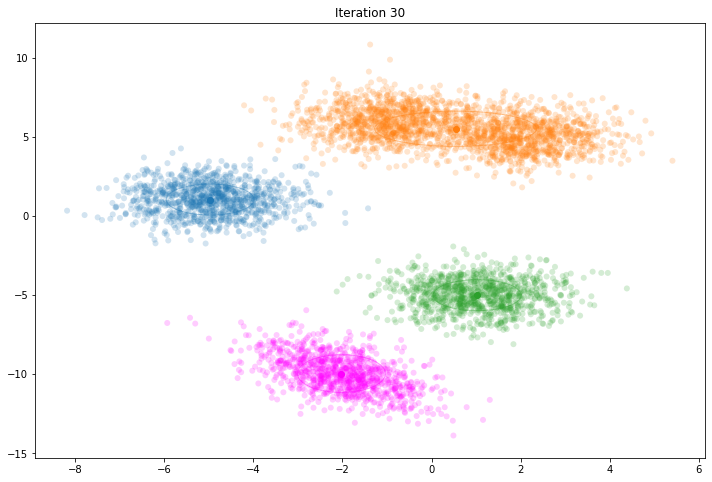
\includegraphics[scale=0.4]{MLE_iter_30.png}
\caption{The MLE algorithm in the 30 iteration, after convergence.}
\label{fig:MLE_3}
\end{figure}

\newpage
%%%%%%%%%%%%%%%%%%%%%%%%%%%%%%%%
\textbf{Over iris data set 3D projection:}

\begin{figure}[h!]
\centering
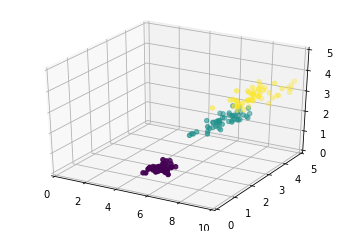
\includegraphics[scale=0.5]{MLE_iris_3D.png}
\caption{The Original Iris 3D data set with first second and third features.}
\label{fig:iris_3d_1}
\end{figure}

\begin{figure}[h!]
\centering
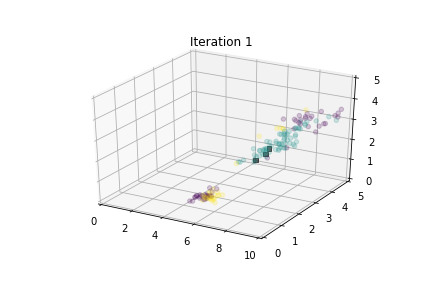
\includegraphics[scale=0.5]{MLE_iris_3D_1_iter.png}
\caption{The initialize centers in the Iris 3D data set for the MLE.}
\label{fig:iris_3d_2}
\end{figure}

\begin{figure}[h!]
\centering
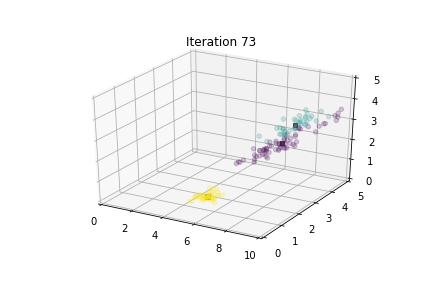
\includegraphics[scale=0.5]{MLE_iris_3D_73_iter.png}
\caption{The MLE after convergence at the 73 iter.}
\label{fig:iris_3d_3}
\end{figure}

\newpage
%%%%%%%%%%%%%%%%%%%%%%%%%%%%%%%%
\textbf{Over iris data set 2D projection using PCA:}

\begin{figure}[h!]
\centering
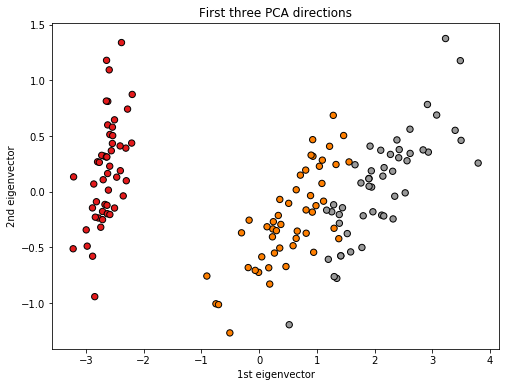
\includegraphics[scale=0.3]{iris_with_PCA_2_eigenvectors.png}
\caption{The projection 2D using PCA of iris data set.}
\label{fig:iris_PCA_1}
\end{figure}

\begin{figure}[h!]
\centering
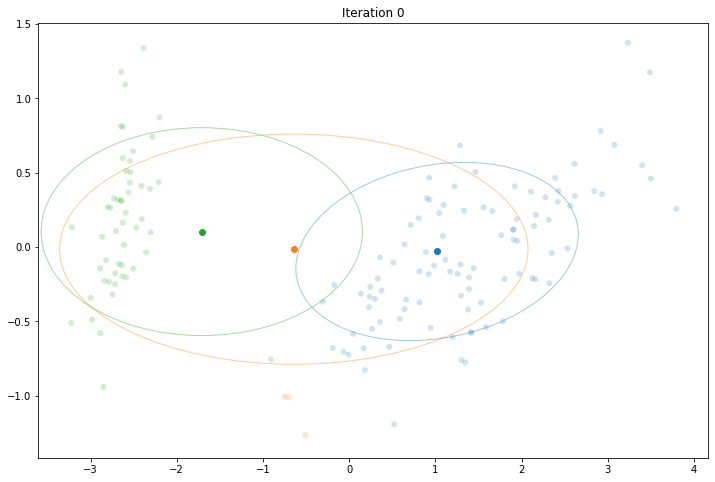
\includegraphics[scale=0.3]{iris_PCA_iter_1.png}
\caption{The initialize centers in the Iris 2D data set for the MLE.}
\label{fig:iris_PCA_2}
\end{figure}

\begin{figure}[h!]
\centering
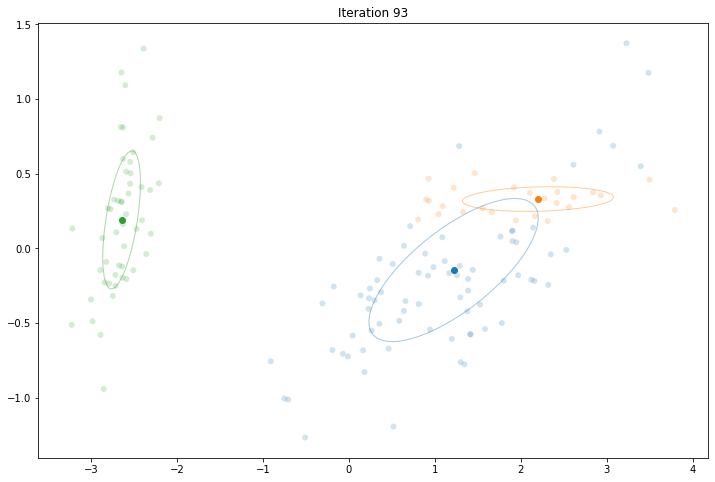
\includegraphics[scale=0.3]{iris_PCA_94.png}
\caption{The MLE after convergence at the 94 iter.}
\label{fig:iris_PCA_3}
\end{figure}


\newpage
%%%%%%%%%%%%%%%%%%%%%%%%%%%%%%%%

\textbf{FAIL CASE - Circular data set:}

\begin{figure}[h!]
\centering
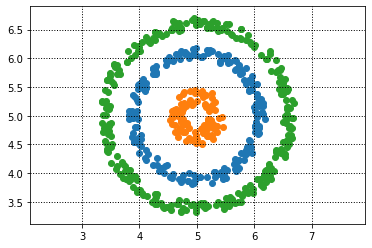
\includegraphics[scale=0.5]{circle.png}
\caption{Try to model 3 circles using MLE Gaussian model.}
\label{fig:Circular_1}
\end{figure}

\begin{figure}[h!]
\centering
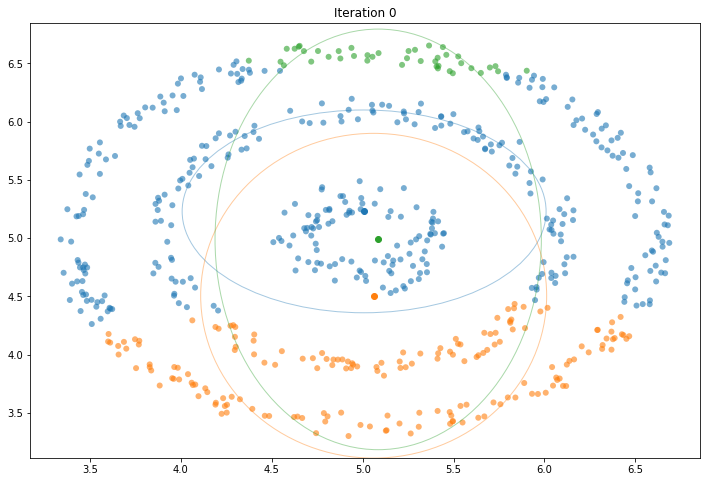
\includegraphics[scale=0.3]{MLE_cir_iter1.png}
\caption{The initialize centers in the circular data set for the MLE.}
\label{fig:Circular_2}
\end{figure}

\begin{figure}[h!]
\centering
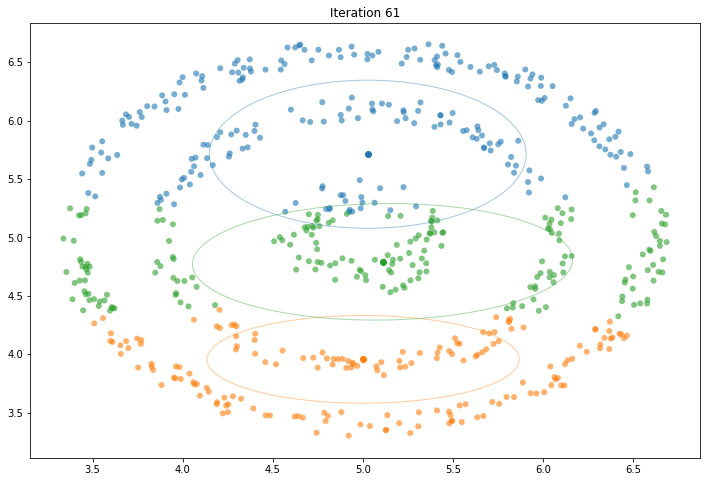
\includegraphics[scale=0.3]{MLE_cir_iter_61.png}
\caption{The MLE after convergence at the 61 iter.}
\label{fig:Circular_3}
\end{figure}

\newpage
%%%%%%%%%%%%%%%%%%%%%%%%%%%%%%%%
\subsection*{MLE Pros and Cons:}

\textbf{Pros:}
\begin{itemize}
    \item Very useful on large data sets.
    \item Good performances 
    \item The best for known Gaussian distributed data. 
\end{itemize} 
\\\\
\textbf{Drowbacks:}
\begin{itemize}
    \item Limited to only gaussians, so cannot use for flexible data.
    \item Need to know ahead who is k.
    \item The statistical inference of the maximun likelihood needed large amount of data so the postirior distributions would be clouse to the data. 
    \item Maximum likelihood estimates can be heavily biased for small samples. The optimality properties may not apply for small samples.
    \item Maximum likelihood can be sensitive to the choice of starting values.
\end{itemize}


\section*{Assignment 2 - Unsupervised Optimal Fuzzy Clustering}

The UOFC \citep{UOFC} estimates both number of clusters and the fuzzy classification of data points to the clusters. In the classical set theory (aka: the MLE we saw before) an element either belongs or does not belong to the cluster. \\ Fuzzy set theory permits the gradual assessment of the membership of elements in a set/cluster. This is described with the aid of a membership function valued in the real unit interval $[0,1]$. \\ 
In UOFC uses incremental approach in order to estimate number of clusters. In each step starting from k = 1 we evaluate the best assignment of the data to the k clusters. To measure how good the k clusters explain the data, We use 6 criterion measurements, the k with the best score is considered to be right k. \\
\textbf{The Clustering Validation Criterion:}
\begin{itemize}
    \item HPV - Hyper Planar Volume: \\ The sum of hyper volumes of each cluster in the data set, we wish to minimize it. 
    \item PDC - Partition Density Central: \\ The density of each cluster determined by the clusters centers, we wish to maximize it.
    \item PDM - Partition Density Maximal: \\ The density of each cluster determined by the maximal membership values in each cluster, we wish to maximize it.
    \item APDC - Average Partition Density Central members: \\ The Average PDC depend on number of clusters, we wish to maximize it just like PDC. 
    \item APDM - Average Partition Density Maximal members: \\ The Average PDM depend on number of clusters, we wish to maximize it just like PDM. 
    \item NPIC - Normalized partition index criteria 
    \item INV - Invariant Criteria: \\ The sum of the hyper volumes normalized by the hyper volume of the data set. we would like to minimized it.
    \item J Criteria: \\ The cost function of the fuzzy C-mean, Trade-off between sparse clusters Concentration and high density clusters, we want to minimized it. 
\end{itemize}

\begin{algorithm}
{\fontsize{10pt}{10pt}\selectfont
\caption{Unsupervised Optimal Fuzzy Clustering}\label{alg:BrothForce}
\begin{algorithmic}[1]
\State $k = 1$
\State q = 3 controls the fuzziness
\State Initialize the first center $c_{1}$ to be the mean of the data.
\While {Run until convergence}
\State \textbf{If} we are in the first iteration \textbf{do}

Initialize $U_{k}$ the membership matrix given the canter $c_{1}$.
\State \textbf{Else} Add another center to the membership matrix $U_{k}$ and 

initialize it with equal distance from all the data points. 

k = k + 1
\State centers, $U_{k}$ = \textbf{calculate fuzzy K mean}(k, data, centers, q, $U_{k}$)
\State centers, $U_{k}$ = \textbf{calculate fuzzy MLE}(k, data, centers, q, $U_{k}$)
\State Calculate fuzzy co-variance matrix $F_{k}$ 
\State Compute HPV, PDC, PDM, APDC, APDM, NPIC, INV, J\_D using $F_{k}$.
\EndWhile 
\end{algorithmic}
}
\end{algorithm} 

\newpage
%%%%%%%%%%%%%%%%%%%%%%%%%%%%%%%%
\subsection*{Results}
\textbf{Over 2D data points randomly drawn from 5 Gaussian’s:}

\begin{figure}[h!]
\centering
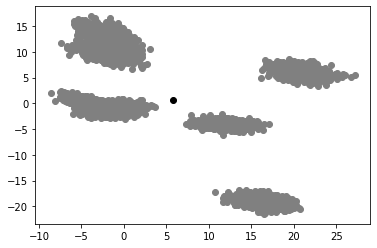
\includegraphics[scale=0.7]{init_gaussians_UOFC.png}
\caption{The UOFC initialization.}
\label{fig:Circular_3}
\end{figure}

\begin{figure}[h!]
\centering
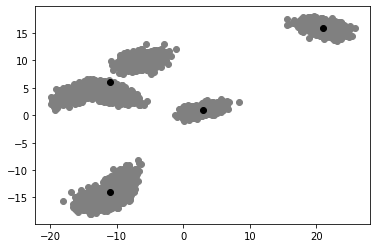
\includegraphics[scale=0.7]{UOFC_gaussians.png}
\caption{The UOFC centers with k = 5 the best k in sense of the criteria.}
\label{fig:Circular_3}
\end{figure}

\newpage
%%%%%%%%%%%%%%%%%%%%%%%%%%%%%%%%

\begin{figure}[h!]
\centering
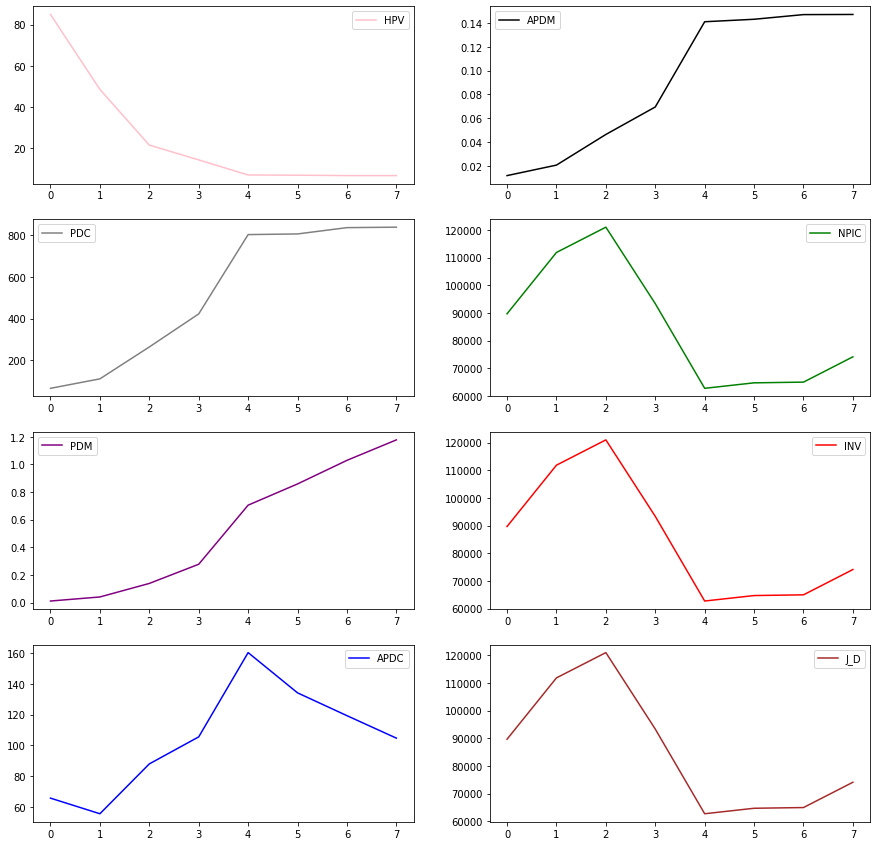
\includegraphics[scale=0.4]{UOFC_gaussians_plot.png}
\caption{All the criteria depending on k.}
\label{fig:Circular_3}
\end{figure}

\newpage
%%%%%%%%%%%%%%%%%%%%%%%%%%%%%%%%


\textbf{Over iris data set 2D projection using PCA:}

\begin{figure}[h!]
\centering
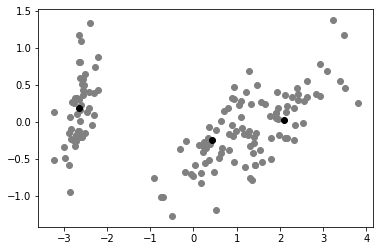
\includegraphics[scale=0.7]{iris_best_pca_uofc.png}
\caption{The UOFC results using 2 centers, the best in sense of criteria.}
\label{fig:Circular_3}
\end{figure}

\begin{figure}[h!]
\centering
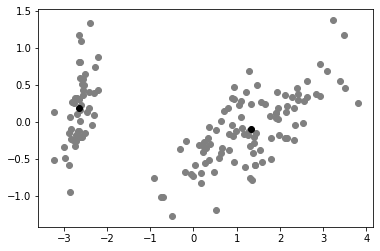
\includegraphics[scale=0.7]{iris_best_2_pca_uofc.png}
\caption{The UOFC results using 3 centers.}
\label{fig:Circular_3}
\end{figure}

\newpage
%%%%%%%%%%%%%%%%%%%%%%%%%%%%%%%%

\begin{figure}[h!]
\centering
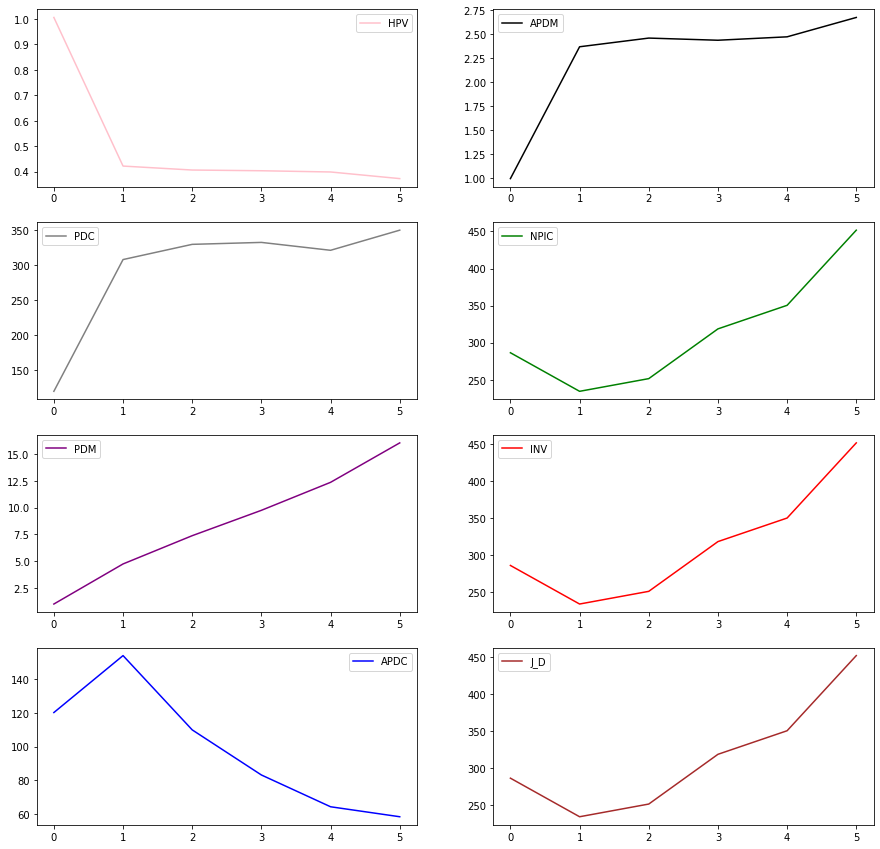
\includegraphics[scale=0.4]{iris_pca_plot_uofc.png}
\caption{All the criteria depending on k.}
\label{fig:Circular_3}
\end{figure}

\newpage
%%%%%%%%%%%%%%%%%%%%%%%%%%%%%%%%

\textbf{Iris projection over the first 2 features:}

\begin{figure}[h!]
\centering
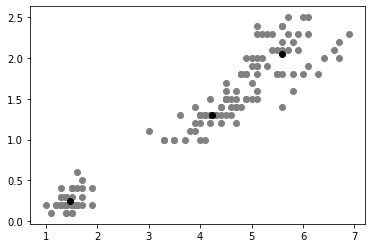
\includegraphics[scale=0.5]{best_iris_2D_uofc.png}
\caption{The best results given the criteria is k = 3}
\label{fig:Circular_3}
\end{figure}


\begin{figure}[h!]
\centering
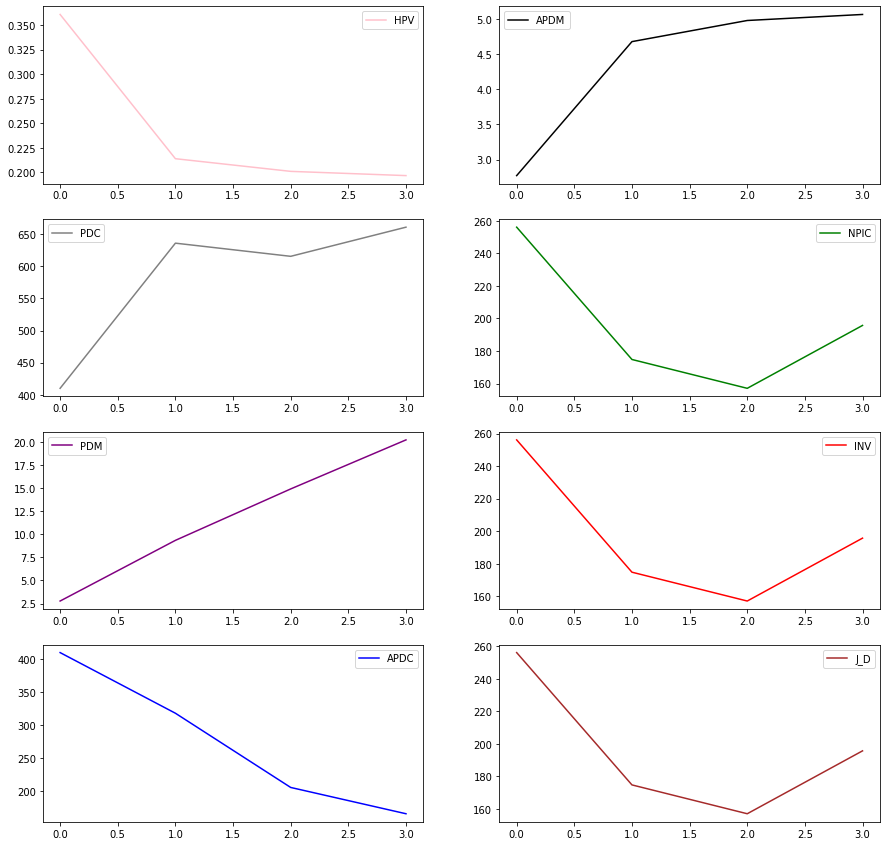
\includegraphics[scale=0.4]{plot_iris_2D_uofc.png}
\caption{All the criteria depending on k.}
\label{fig:Circular_3}
\end{figure}


\newpage
%%%%%%%%%%%%%%%%%%%%%%%%%%%%%%%%


\textbf{FAIL CASE- Circular data set:}

\begin{figure}[h!]
\centering
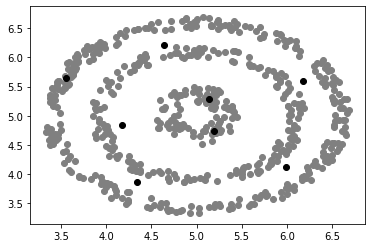
\includegraphics[scale=0.5]{cir_uofc.png}
\caption{The results given k = 8}
\label{fig:Circular_3}
\end{figure}


\begin{figure}[h!]
\centering
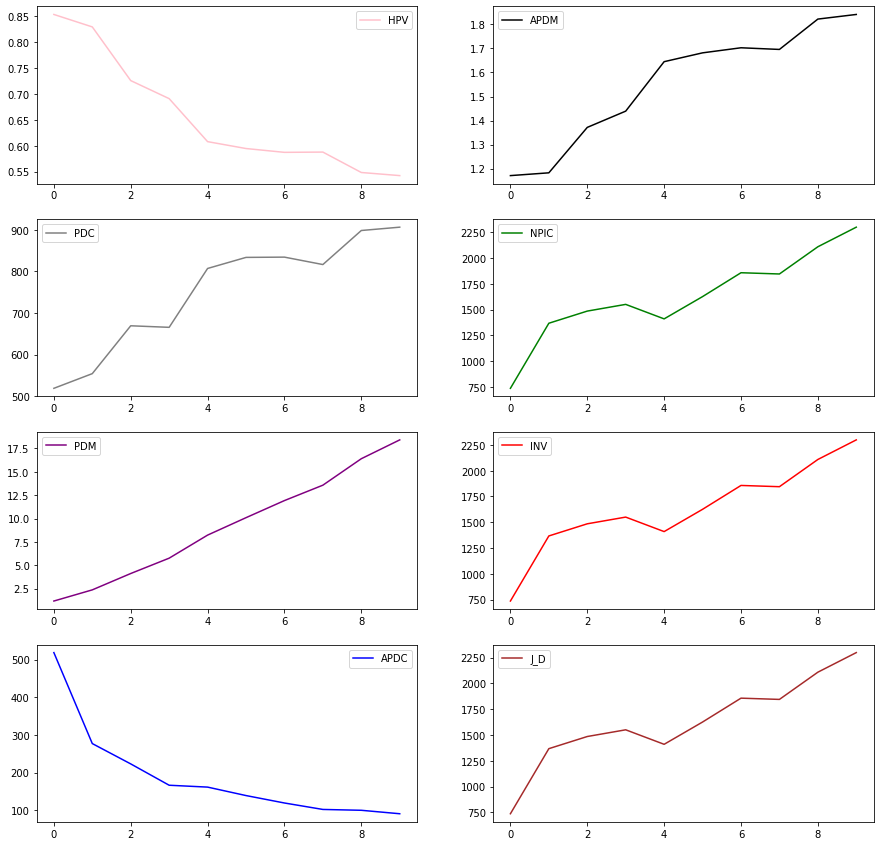
\includegraphics[scale=0.4]{circle_uofc.png}
\caption{All the criteria depending on k.}
\label{fig:Circular_3}
\end{figure}

\newpage
%%%%%%%%%%%%%%%%%%%%%%%%%%%%%%%%
\subsection*{UOFC Pros and Cons:}

\textbf{Pros:}
\begin{itemize}
    \item Fuzzy clustering very sensitive to initialization UOFC not that much. 
    \item Don't need to know k ahead. 
\end{itemize}\\
\textbf{Drawbacks:}
\begin{itemize}
    \item Needed to scale q - fuzziness parameters.
    \item Out layers data points also part of the clusters calculation. 
    \item not good for not circular data. 
\end{itemize}

\newpage
%%%%%%%%%%%%%%%%%%%%%%%%%%%%%%%%
\section*{Assignment 3 - Agglomerative Hierarchical Clustering}
The agglomerative clustering also known as Agglomerative Nesting is the most common type of hierarchical clustering used to group objects in clusters based on their similarity. Agglomerative clustering works in a “bottom-up” manner. That is, each object is initially considered as a single-element cluster (leaf). At each step of the algorithm, the two clusters that are the most similar are combined into a new bigger cluster (nodes). This procedure is iterated until all points are member of just one single big cluster (root). \\

\begin{algorithm}
{\fontsize{10pt}{10pt}\selectfont
\caption{Agglomerative Hierarchical Clustering}\label{alg:BrothForce}
\begin{algorithmic}[1]
\State Initialize k number of clusters = n number of data points.
\State Initialize $\forall i = \{1,...,n\} : D_{i} = \{X_{i}\} $ each cluster D contains only one data point. 
\While {$c > 1$}
\State Find the nearest clusters for example: $D_{i}, D_{j}$ 
\State Merge $D_{i}, D_{j}$ to be one cluster.
\State c = c - 1 
\EndWhile 
\end{algorithmic}
}
\end{algorithm}  

We tested 4 different types of distance measures for the nearest clusters.
For all $x_{i} \in D_{i}, x_{j} \in D_{j}$ we calculate the distance between $D_{i}, D_{j}$ as follow: 
\begin{itemize}
    \item $d_{min}(D_{i}, D_{j}) = min_{x \in D_{i}, x' \in D_{j}} ||x-x'||$
    \item $d_{max}(D_{i}, D_{j}) = max_{x \in D_{i}, x' \in D_{j}} ||x-x'||$
    \item $d_{avg}(D_{i}, D_{j}) = \frac{1}{n_{i}n_{j}} \Sigma_{x \in D_{i}} \Sigma_{x' \in D_{j}} ||x-x'||$
    \item $d_{mean}(D_{i}, D_{j}) = ||m_{i}-m_{j}||$
\end{itemize}

\subsection*{Results}
\textbf{Data points Drown from 6 Gaussian's:}

\begin{figure}[h!]
\centering
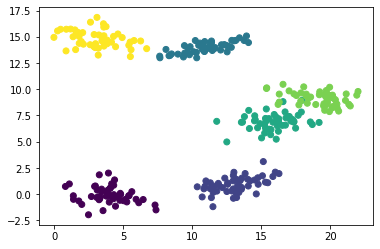
\includegraphics[scale=0.4]{hir_6_gaussians.png}
\caption{The data points original labels.}
\label{fig:hir_gus_1}
\end{figure}

\newpage
%%%%%%%%%%%%%%%%%%%%%%%%%%%%%%%%

\begin{figure}[h!]
\centering
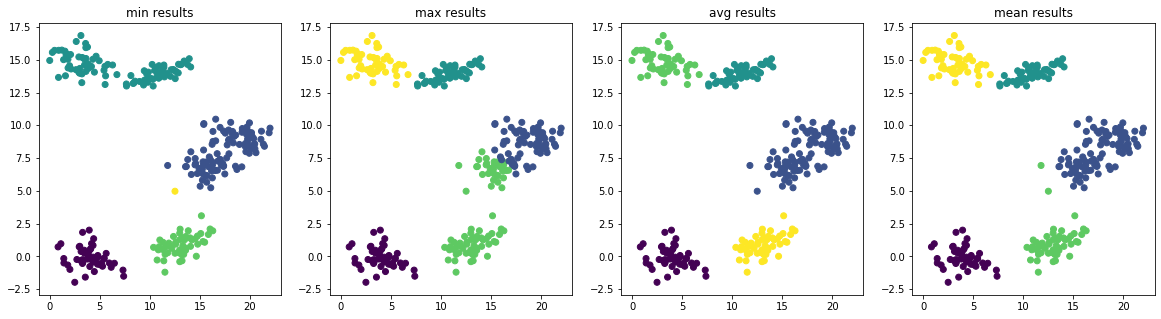
\includegraphics[scale=0.4]{hir_6_gaussians_5.png}
\caption{The results of all 4 methods when c = 5, there are 5 clusters.}
\label{fig:hir_gus_2}
\end{figure}


\begin{figure}[h!]
\centering
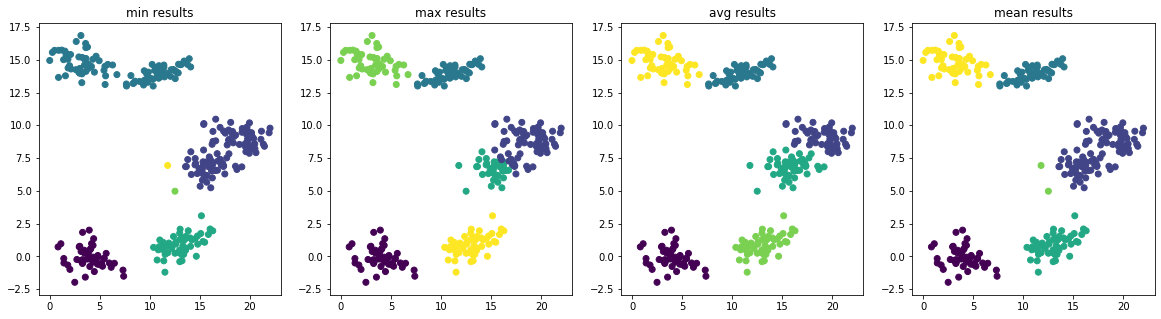
\includegraphics[scale=0.4]{hir_6_gaussians_6.png}
\caption{The results of all 4 methods when c = 6, there are 6 clusters. As you can see the best results is given by the avg distance.}
\label{fig:hir_gus_3}
\end{figure}



\textbf{Iris data set:}

\begin{figure}[h!]
\centering
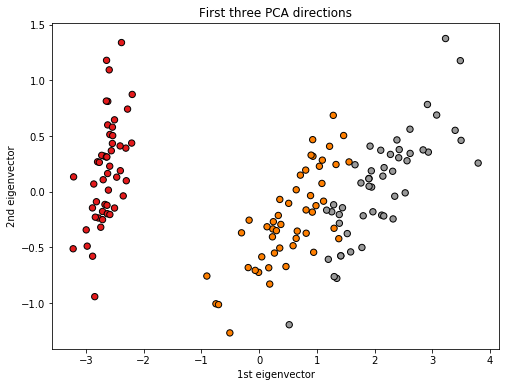
\includegraphics[scale=0.4]{iris_pca_hir.png}
\caption{The iris data set in 2D using PCA and taking the two biggest eigenvalues.}
\label{fig:Circular_3}
\end{figure}

\newpage
%%%%%%%%%%%%%%%%%%%%%%%%%%%%%%%%

\begin{figure}[h!]
\centering
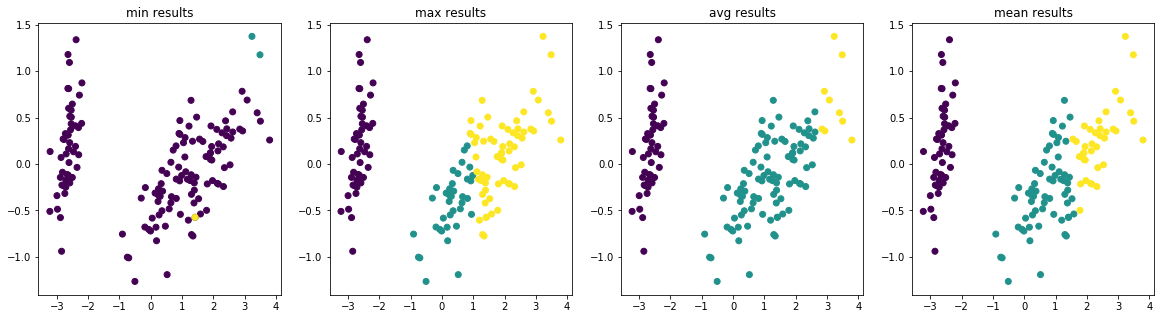
\includegraphics[scale=0.4]{iris_hir_3.png}
\caption{The results of all the methods, the best results is between max and mean. The worst result is min criteria.}
\label{fig:Circular_3}
\end{figure}

\textbf{Circular data set:}

\begin{figure}[h!]
\centering
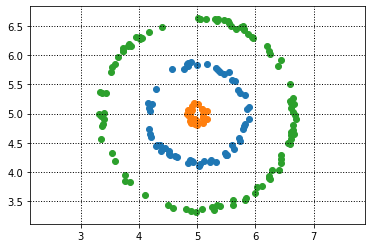
\includegraphics[scale=0.4]{cir_hir_init.png}
\caption{The circular data set.}
\label{fig:Circular_3}
\end{figure}


\begin{figure}[h!]
\centering
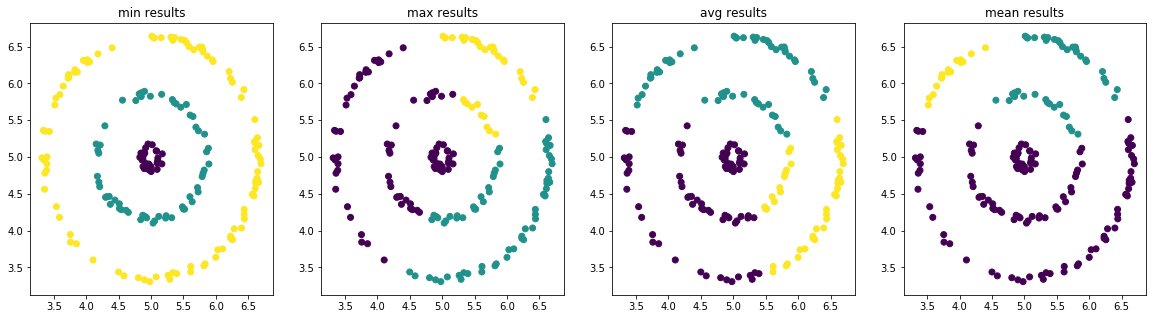
\includegraphics[scale=0.4]{cir_hir.png}
\caption{The only distance criteria that manage to find the circles is the minimum criteria, and it only work if the distance between the circles is big enough.}
\label{fig:Circular_3}
\end{figure}


\newpage
%%%%%%%%%%%%%%%%%%%%%%%%%%%%%%%%

\subsection*{AHC Pros and Cons:}

\textbf{Pros:} 
\begin{itemize}
    \item Best for capturing clusters of different sizes and shapes
    \item Computationally possible for large datasets
\end{itemize}
\textbf{Drowbacks:}

\begin{itemize}
    \item Sensitive to the method selection.
    \item sensitive to noise.
    \item complete link and group average are not affected by noise, but have a bias towards finding global patterns.
    \item Doesn't give good results for large data sets because it uses too little information.
\end{itemize}

\newpage
%%%%%%%%%%%%%%%%%%%%%%%%%%%%%%%%

\section*{Assignment 4 - "The Chinese restaurant process" Dirichlet Process Gaussian Mixture Model:}

Bayesian nonparametric (BNP) models approach is to fit a single model that can adapt its complexity to the data and allow the complexity to grow as more data are observed. \\
The BNP approach finesses the problem of choosing the number of clusters by assuming that it is infinite, while specifying the prior over infinite groupings $P(c)$ in such a way that it favors assigning data to a small number of groups. The prior over groupings is called the Chinese Restaurant Process (CRP). \\
Imagine a restaurant with an infinite number of tables, and imagine a sequence of customers entering the restaurant and sitting down. \\
The first customer enters and sits at the first table. \\ The second customer enters and sits at the first table with probability $\frac{1}{1+\alpha}$, and the second table with probability $\frac{\alpha}{1+\alpha}$, where $\alpha$ is a positive real and called the concentration parameter. \\
More formally, let $c_{n}$ be the table assignment of the $n$th customer. The probability he/she will sit in the $k$th table is given by the following probability:

\[
    P(c_{n} = k|c_{1:n-1}) =
    \left\{
        \begin{array}{ll}
          \textbf{if } k \leq K_{+}: \
          \frac{m_{k}}{n-1+\alpha} \\
          \textbf{(i.e k is a previously occupied table)} \\
          \textbf{otherwise: }
          \frac{\alpha}{n-1+\alpha} \\
          \textbf{(i.e k is the next unoccupied table)}
        \end{array}
    \right.
  \]
Where $m_{k}$ is the number of customers sitting at table k, and $K_{+}$ is the number of tables for which $m_{k} > 0 $. Intuitively, a larger value of $\alpha$ will produce more occupied tables (and fewer customers per table).\\\\
\textbf{Dirichlet Process Gaussian Mixture Model:} \\
The Dirichlet process (DP) is a distribution over distributions. It is parameterized by a concentration parameter $\alpha > 0 $ and a base distribution $G_{0}$, which is a distribution over a space $\Theta$. A random distribution G drawn from a DP is denoted by $G \sim DP(\alpha, G_{0})$. One property of the Dirichlet process \citep{ferguson1973} is that random distributions drawn from the Dirichlet process are discrete and called "atoms". \\\\
$G = \Sigma^{\infty}_{k=1} \pi_{k}\delta_{\theta_{k}^{*}}$ \\\\
Where $\pi_{k}$ is the probability assigned to the $k$th atom and $\delta_{\theta_{k}^{*}}$ is the location or value of that atom, and these atoms are drawn independently from the base distribution $G_{0}$. \\\\
The second property connects the Dirichlet process to the Chinese restaurant process. Consider a random distribution drawn from a DP followed by repeated draws from that random distribution, \\\\
$G \sim DP(\alpha, G_{0})$ \\
$\theta_{i} \sim G \ \ \ i \in \{1,...,n\}$ \\\\
The joint distribution of $\theta_{1:n}$, which is
obtained by marginalizing out the random distribution G is , \\\\
$p(\theta_{1},...,\theta_{n}|\alpha,G_{0}) = \int \left( \Pi^{n}_{i=1} p(\theta_{i}|G) \right) dP(G|a,G_{0})$ \\\\
Ferguson (1973) \citep{ferguson1973} showed that, under this joint distribution, the $\theta_{i}$ will exhibit a
clustering property — they will share repeated values with positive probability. (Note that, for example, repeated draws from a Gaussian do not exhibit this property.) The structure of shared values defines a partition of the integers from 1 to n, and the distribution of this partition is a Chinese restaurant process with parameter $\alpha$. Finally, he showed that the unique values of $\theta_{i}$ shared among the variables are independent draws from $G_{0}$. \\ 
A DP mixture adds a third step to the model above \citep{Antoniak1974MixturesOD}: \\\\
$G \sim DP(\alpha, G_{0})$ \\
$\theta_{i} \sim G \ \ \ i \in \{1,...,n\}$ \\
$x_{i} \sim p(\dot|\theta_{i})$ \\\\
Marginalizing out G reveals that the DP mixture is equivalent to a CRP mixture. Good Gibbs sampling algorithms for DP mixtures are based on this representation. \\\\
\textbf{The stick-breaking construction of DP \citep{sethuraman1994constructive}:} \\
Consider a stick with unit length. We divide the stick into an infinite number of segments $\pi_{k}$ by the following process. First, choose a beta random variable $\beta_{1} \sim Beta(1,\alpha)$ and break of $\beta_{1}$ of the stick. For each remaining segment, choose another beta distributed random variable, and break off that proportion of the remainder of the stick. This gives us an infinite collection of weights $\pi_{k}$, \\\\
$\beta_{k} \sim Beta(1,\alpha)$ \\
$\pi_{k} = \beta_{k} \Pi_{j=1}^{k-1} (1-\beta_{j}) \ \ k = 1,2,3,...$ \\\\
Finally, we construct a random distribution using \\\\
$G = \Sigma^{\infty}_{k=1} \pi_{k}\delta_{\theta_{k}^{\star}}$ ,\\\\ where we take an infinite number of draws from a base distribution $G_{0}$ and draw the weights as in the second equation. Sethuraman \citep{sethuraman1994constructive} showed that the distribution of this random distribution is a $DP(\alpha, G_{0})$.
This representation of the Dirichlet process, and its corresponding use in a Dirichlet process mixture, allows us to compute a variety of functions of posterior DPs \citep{gelfand2002computational} and is the basis for the variational approach to approximate inference. 


\subsection*{DPGMM Pros and Cons:}

\textbf{Pros:} 
\begin{itemize}
    \item Very stable to changes of the parameters, leading to more stability and less tuning.
    \item We do not need to know the number of clusters. 
\end{itemize}

\textbf{Drowbacks:}

\begin{itemize}
    \item the extra parametrization can and will make inference slower, although not by much.
    \item There are many implicit biases in the Dirichlet process and the inference algorithms, and whenever there is a mismatch between these biases and the data it might be possible to fit better models using a finite mixture.
\end{itemize}


\newpage
%%%%%%%%%%%%%%%%%%%%%%%%%%%%%%%%

\subsection*{Results}
\textbf{Iris 2D data set:}
\begin{figure}[h!]
\centering
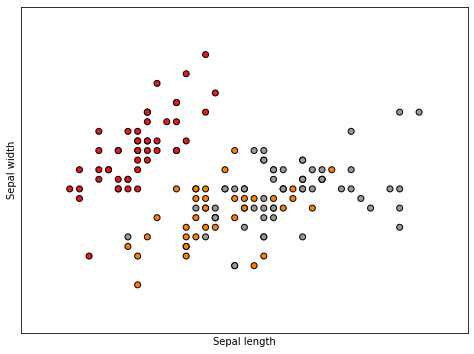
\includegraphics[scale=0.5]{iris_data.png}
\caption{The iris 2D data set.}
\label{fig:DPGMM1}
\end{figure}


\begin{figure}[h!]
\centering
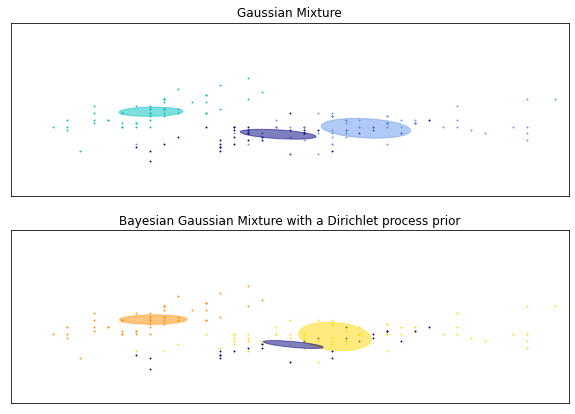
\includegraphics[scale=0.6]{iris_DPGMM_init.png}
\caption{The results of the DPGMM over iris data set vs of gaussian mixture model.}
\label{fig:Circular_3}
\end{figure}

\newpage
%%%%%%%%%%%%%%%%%%%%%%%%%%%%%%%%

\textbf{Iris 3D data set:}

\begin{figure}[h!]
\centering
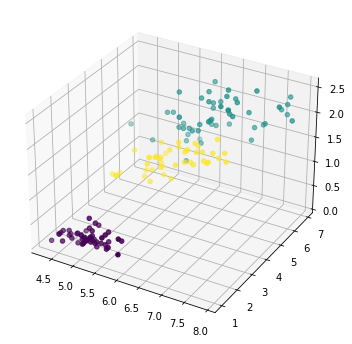
\includegraphics[scale=0.4]{iris_3D_DPGMM.png}
\caption{The iris data set with the the first third and forth values.}
\label{fig:Circular_3}
\end{figure}

\begin{figure}[h!]
\centering
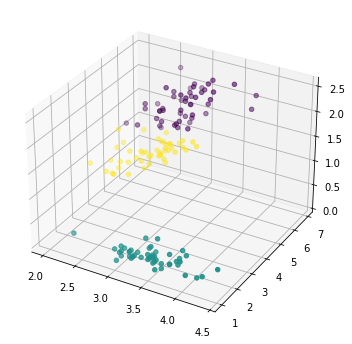
\includegraphics[scale=0.4]{DPGMM_iris_1_2_3.png}
\caption{The results of the \textbf{DPGMM} over iris data set, almost prefect!.}
\label{fig:Circular_3}
\end{figure}

\begin{figure}[h!]
\centering
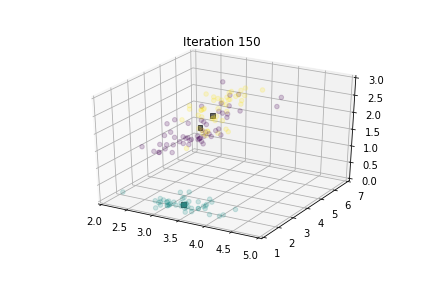
\includegraphics[scale=0.5]{comp_MLE_DPGMM.png}
\caption{The results of the GMM over iris data set. For comparison.}
\label{fig:Circular_3}
\end{figure}

\newpage
%%%%%%%%%%%%%%%%%%%%%%%%%%%%%%%%

\textbf{Circular data set:}

\begin{figure}[h!]
\centering
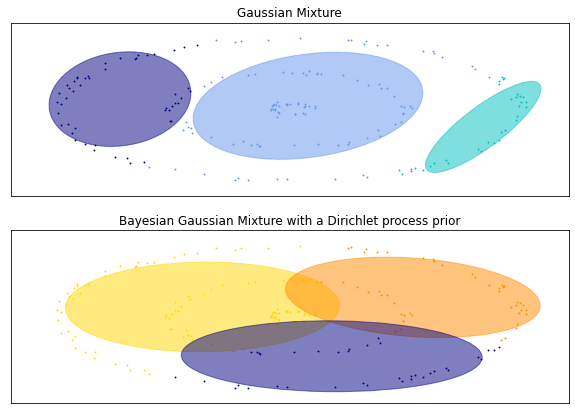
\includegraphics[scale=0.5]{cir_DPGMM.png}
\caption{The results the circular data set with both DPGMM and GMM.}
\label{fig:Circular_3}
\end{figure}


\textbf{Random Gaussian data set:}

\begin{figure}[h!]
\centering
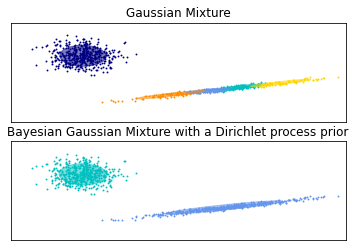
\includegraphics[scale=0.9]{DPGMM.png}
\caption{The results of DPGMM and GMM over random Gaussian data set.}
\label{fig:Circular_3}
\end{figure}

\newpage
%%%%%%%%%%%%%%%%%%%%%%%%%%%%%%%%% 

\bibliographystyle{plain}
\bibliography{references}
\end{document}
